% ============================================================
% Lecture deck — Module 14 / Notebook 43
% Digital Transformation & AI-Induced Change
% HSBI house style (Prof. Dr. Christoph Weisser). English content.
% Thin lecture deck with native TikZ visuals — the notebook is the
% single source of truth.
% ============================================================
\documentclass[aspectratio=169,11pt]{beamer}

\usepackage[utf8]{inputenc}
\usepackage[T1]{fontenc}
\usepackage{lmodern}
\usepackage[english]{babel}
\usepackage{graphicx}
\usepackage{booktabs}
\usepackage{amsmath,amssymb}
\usepackage{xcolor}
\usepackage{tikz}
\usetikzlibrary{positioning,arrows.meta,shapes.geometric,calc,fit,backgrounds}

\usetheme{Madrid}
\usecolortheme{default}
\setbeamertemplate{navigation symbols}{}
\setbeamertemplate{footline}[frame number]
\setbeamertemplate{blocks}[rounded][shadow=false]
\setbeamertemplate{headline}{%
  \leavevmode%
  \hbox{%
    \begin{beamercolorbox}[wd=\paperwidth,ht=2.5ex,dp=1.125ex]{section in head/foot}%
      \insertsectionnavigationhorizontal{\paperwidth}{}{\hskip0pt plus1filll}%
    \end{beamercolorbox}%
  }%
}
\AtBeginSection[]{%
  \begin{frame}{Outline}
    \tableofcontents[currentsection,sectionstyle=show/shaded,subsectionstyle=show/show/hide]
  \end{frame}
}

% ---- Accent palette (matches the notebooks' matplotlib palette) ----
\definecolor{hsbiblue}{RGB}{45,57,120}
\definecolor{hsbimid}{RGB}{76,114,176}
\definecolor{hsbilight}{RGB}{225,231,247}
\definecolor{cgreen}{RGB}{85,164,103}
\definecolor{corange}{RGB}{221,132,82}
\definecolor{cred}{RGB}{196,78,82}
\definecolor{cpurple}{RGB}{129,114,178}
\tikzset{
  box/.style={rounded corners=3pt, draw=hsbiblue, line width=1pt, fill=hsbilight, align=center, inner sep=5pt, font=\footnotesize},
  stair/.style={rounded corners=3pt, draw=hsbiblue, line width=1.1pt, fill=hsbilight, align=center, text width=2.3cm, minimum height=0.95cm, font=\scriptsize},
  arr/.style={-{Stealth[length=2.6mm]}, line width=1pt, draw=hsbiblue},
}

\title{Digital Transformation \& AI-Induced Change}
\subtitle{Module 14 --- Business AI in Practice $\cdot$ Notebook 43}
\author{Prof.\ Dr.\ Christoph Weisser}
\institute{HSBI}
\date{Summer Semester 2026}

\begin{document}

\begin{frame}\titlepage\end{frame}

\begin{frame}{Contents}
  \tableofcontents[hideallsubsections]
\end{frame}

% ============================================================
\section{Why now}
% ============================================================
\begin{frame}{Why AI feels different \emph{this} time}
  \begin{center}
  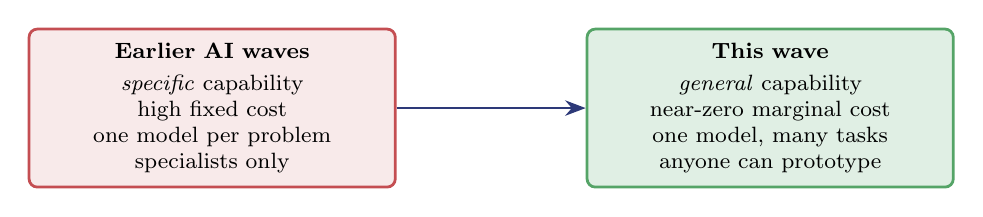
\begin{tikzpicture}
    \node[box, fill=cred!12, draw=cred, text width=4.3cm] (old)
      {\textbf{Earlier AI waves}\\[2pt] \emph{specific} capability\\ high fixed cost\\ one model per problem\\ specialists only};
    \node[box, fill=cgreen!18, draw=cgreen, text width=4.3cm, right=2.4cm of old] (new)
      {\textbf{This wave}\\[2pt] \emph{general} capability\\ near-zero marginal cost\\ one model, many tasks\\ anyone can prototype};
    \draw[arr] (old) -- (new);
  \end{tikzpicture}
  \end{center}
  \begin{itemize}
    \item \textbf{Cheap intelligence} --- an LLM call costs cents and needs no in-house ML team.
    \item \textbf{Natural-language interface} --- an organisational change, not just a technical one.
  \end{itemize}
\end{frame}

% ============================================================
\section{Tasks}
% ============================================================
\begin{frame}{The unit of change: tasks, not jobs}
  \begin{itemize}
    \item A job is a \emph{bundle of tasks}. AI absorbs \emph{tasks}, rarely whole jobs.
    \item Enumerate the tasks; score each; start where the win is safe and easy.
  \end{itemize}
  \begin{exampleblock}{Reframe the stakeholder question}
    ``Will AI replace these 12 people?'' $\;\to\;$ ``Which of their \emph{tasks} will AI absorb, and what do the people do with the freed-up time?''
  \end{exampleblock}
\end{frame}

\begin{frame}{Where AI lands first --- patternable $\times$ stakes}
  \begin{center}
  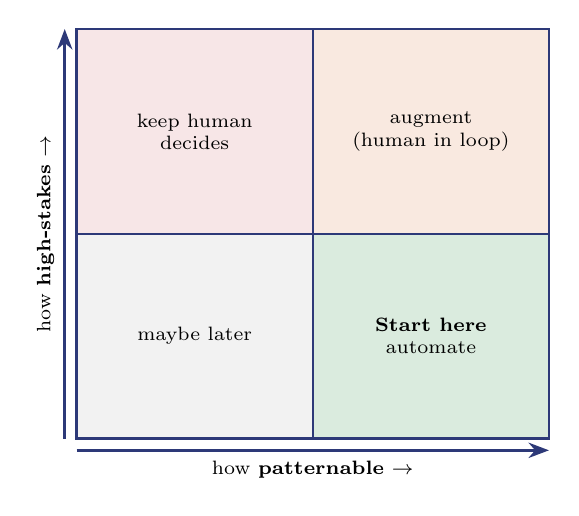
\begin{tikzpicture}[scale=1]
    % quadrant fills
    \fill[cgreen!22]  (3,0) rectangle (6,2.6);
    \fill[corange!18] (3,2.6) rectangle (6,5.2);
    \fill[gray!10]    (0,0) rectangle (3,2.6);
    \fill[cred!14]    (0,2.6) rectangle (3,5.2);
    % grid + axes
    \draw[hsbiblue,line width=1pt] (0,0) rectangle (6,5.2);
    \draw[hsbiblue,line width=0.6pt] (3,0)--(3,5.2);
    \draw[hsbiblue,line width=0.6pt] (0,2.6)--(6,2.6);
    \draw[arr] (0,-0.15) -- (6,-0.15) node[midway,below,font=\scriptsize]{how \textbf{patternable} $\to$};
    \draw[arr] (-0.15,0) -- (-0.15,5.2) node[midway,above,rotate=90,font=\scriptsize]{how \textbf{high-stakes} $\to$};
    % labels
    \node[align=center,font=\scriptsize\bfseries] at (4.5,1.3) {Start here\\ \scriptsize\mdseries automate};
    \node[align=center,font=\scriptsize] at (4.5,3.9) {augment\\ (human in loop)};
    \node[align=center,font=\scriptsize] at (1.5,1.3) {maybe later};
    \node[align=center,font=\scriptsize] at (1.5,3.9) {keep human\\ decides};
  \end{tikzpicture}
  \end{center}
  \vspace{-2pt}
  {\footnotesize Begin in the \textbf{high-pattern / low-stakes} corner: cheap to build, cheap to be wrong.}
\end{frame}

% ============================================================
\section{Maturity}
% ============================================================
\begin{frame}{The five-stage AI maturity model}
  \begin{center}
  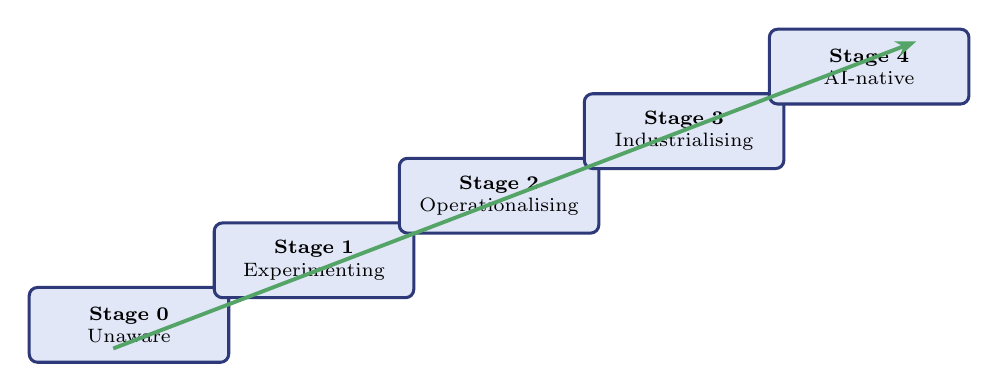
\begin{tikzpicture}
    \foreach \i/\name in {0/Unaware, 1/Experimenting, 2/Operationalising, 3/Industrialising, 4/AI-native}{
      \node[stair] at (\i*2.35, \i*0.82) {\textbf{Stage \i}\\ \name};
    }
    \draw[arr, draw=cgreen, line width=1.4pt] (-0.2,-0.3) -- (10.0,3.6);
  \end{tikzpicture}
  \end{center}
  \vspace{2pt}
  {\footnotesize Most organisations sit between \textbf{1} and \textbf{2}. The model names the \emph{next realistic step} --- not the destination.}
\end{frame}

\begin{frame}{Maturity --- the signature behaviour of each stage}
  \small
  \begin{center}
  \begin{tabular}{clp{6.6cm}}
    \toprule
    \textbf{\#} & \textbf{Stage} & \textbf{Signature behaviour} \\
    \midrule
    0 & Unaware          & Not in the strategy; staff quietly use ChatGPT on their phones. \\
    1 & Experimenting    & A few pilots in a sandbox; results stay in slides. \\
    2 & Operationalising & One or two features live in production, owned by a real team. \\
    3 & Industrialising  & A platform team; reusable infra; a feature ships in weeks. \\
    4 & AI-native        & AI is in the \emph{process design}, not bolted on. \\
    \bottomrule
  \end{tabular}
  \end{center}
\end{frame}

% ============================================================
\section{Strategies}
% ============================================================
\begin{frame}{Three change strategies}
  \begin{center}
  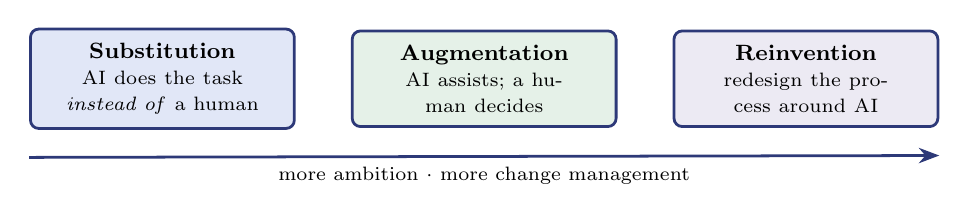
\begin{tikzpicture}
    \node[box, fill=hsbilight, text width=3.0cm] (s) {\textbf{Substitution}\\ \scriptsize AI does the task \emph{instead of} a human};
    \node[box, fill=cgreen!15, text width=3.0cm, right=0.7cm of s] (a) {\textbf{Augmentation}\\ \scriptsize AI assists; a human decides};
    \node[box, fill=cpurple!15, text width=3.0cm, right=0.7cm of a] (r) {\textbf{Reinvention}\\ \scriptsize redesign the process around AI};
    \draw[arr] ($(s.south west)+(0,-0.35)$) -- ($(r.south east)+(0,-0.35)$)
      node[midway,below,font=\scriptsize]{more ambition $\cdot$ more change management};
  \end{tikzpicture}
  \end{center}
  \begin{exampleblock}{Intuition}
    Most real projects are \textbf{augmentation} in year one, drifting to \textbf{substitution} for the well-understood tasks as trust grows.
  \end{exampleblock}
\end{frame}

% ============================================================
\section{Pitfalls}
% ============================================================
\begin{frame}{The five adoption pitfalls --- and how to prevent them}
  \small
  \begin{center}
  \begin{tabular}{lp{6.4cm}}
    \toprule
    \textbf{Pitfall} & \textbf{Prevention} \\
    \midrule
    \textcolor{cred}{\textbf{Solutionism}}        & fix the process \emph{before} you automate it \\
    \textcolor{cred}{\textbf{Pilot purgatory}}    & define a production owner on day one \\
    \textcolor{cred}{\textbf{No monitoring}}       & ship the eval dashboard \emph{with} the feature \\
    \textcolor{cred}{\textbf{No change management}}& budget for adoption, training, incentives \\
    \textcolor{cred}{\textbf{Governance as afterthought}} & put ethics / safety in the first design review \\
    \bottomrule
  \end{tabular}
  \end{center}
  \vspace{2pt}
  {\footnotesize ``92\,\% accurate at launch'' means nothing if nobody is watching the number six months later.}
\end{frame}

% ============================================================
\section{People}
% ============================================================
\begin{frame}{The human side}
  \begin{itemize}
    \item Job descriptions, skill mix, and team shape begin changing the \emph{day you ship}.
    \item Frame the change as augmentation, and give people a one-click override.
  \end{itemize}
  \begin{block}{The cheapest trust intervention}
    Publish the AI's \textbf{confidence score} next to every output. Users quickly learn when to trust it and when to double-check.
  \end{block}
\end{frame}

\begin{frame}{Companion notebook}
  \begin{exampleblock}{This is the conceptual half of the lecture}
    The hands-on judgement --- task inventories, placing an organisation on the maturity model, the pre-mortem, the strategy-map 2$\times$2 --- lives in \textbf{Notebook 43}, with worked solutions.
  \end{exampleblock}
  \begin{itemize}
    \item Prerequisite-free; the course's \emph{spiral} recommends it as an early read (the ``why'').
    \item Next: \textbf{Notebook 44 --- Architecture Patterns}.
  \end{itemize}
\end{frame}

\end{document}
